
\documentclass[journal]{IEEEtran}

\usepackage[backend=biber,style=ieee]{biblatex}

\renewcommand{\tablename}{Tabla} 
\renewcommand{\abstractname}{\large Resumen}
\renewcommand{\IEEEkeywordsname}{\large Palabras Clave}
\renewcommand{\figurename}{Fig.}


\addbibresource{references.bib}

\usepackage[utf8]{inputenc}   % Para acentos y ñ
\usepackage[T1]{fontenc}      % Para acentos correctos en salida PDF
\usepackage{babel}
\usepackage{tikz}
\usetikzlibrary{arrows.meta, positioning}
\usepackage{graphicx}
\usepackage{tabularx}

\usepackage{array}
\usepackage{booktabs}
\usepackage{makecell}
\usepackage{titlesec}

\usepackage[font=footnotesize,labelfont=bf]{caption}
\usepackage{hyperref} % Para enlaces y \url

% *** GRAPHICS RELATED PACKAGES ***
%
\ifCLASSINFOpdf
  % \usepackage[pdftex]{graphicx}
  % declare the path(s) where your graphic files are
  % \graphicspath{{../pdf/}{../jpeg/}}
  % and their extensions so you won't have to specify these with
  % every instance of \includegraphics
  % \DeclareGraphicsExtensions{.pdf,.jpeg,.png}
\else
  % or other class option (dvipsone, dvipdf, if not using dvips). graphicx
  % will default to the driver specified in the system graphics.cfg if no
  % driver is specified.
  % \usepackage[dvips]{graphicx}
  % declare the path(s) where your graphic files are
  % \graphicspath{{../eps/}}
  % and their extensions so you won't have to specify these with
  % every instance of \includegraphics
  % \DeclareGraphicsExtensions{.eps}
\fi



% correct bad hyphenation here
\hyphenation{op-tical net-works semi-conduc-tor}


\begin{document}
%
% paper title
% Titles are generally capitalized except for words such as a, an, and, as,
% at, but, by, for, in, nor, of, on, or, the, to and up, which are usually
% not capitalized unless they are the first or last word of the title.
% Linebreaks \\ can be used within to get better formatting as desired.
% Do not put math or special symbols in the title.
\title{Informe Parcial: Módulo Tracker LoRa/APRS}

\author{Wilberth-Gutierrez Montero,~\IEEEmembership{Estudiante,~Instituto Tecnológico de Costa Rica} \\
        Oscar-Gonzalez Cambronero,~\IEEEmembership{Estudiante,~Instituto Tecnológico de Costa Rica} \\
        Nagel-Mejía Segura,~\IEEEmembership{Estudiante,~Instituto Tecnológico de Costa Rica}
        % <-this % stops a space
}

% The paper headers
\markboth{Taller Integrador, ~EL-5610, ~II-Semestre-2025}%
{Shell \MakeLowercase{\textit{et al.}}: Bare Demo of IEEEtran.cls for IEEE Journals}





% make the title area
\maketitle

% As a general rule, do not put math, special symbols or citations
% in the abstract or keywords.
\begin{abstract}

Este documento recopila información sobre el desarrollo de un módulo Tracker basado en tecnología LoRa/APRS, enfocado en la transmisión y recepción de datos de localización en tiempo real a una página web. Tiene como objetivo abordar detalles técnicos de la implementación, protocolos de comunicación utilizados, definición de tramas y finalmente presenta un breve itinerario de las actividades a realizar para completar el proyecto.

\end{abstract}

% Note that keywords are not normally used for peerreview papers.
\begin{IEEEkeywords}
Trama, modulación, registros, potencia.
\end{IEEEkeywords}


\IEEEpeerreviewmaketitle



\section{Introducción}

\IEEEPARstart{P}{}ara desarrollar un \textit{tracker} capaz de transmitir y recibir datos de localización con múltiples protocolos de comunicación, es necesario integrar diversos componentes electrónicos y módulos de comunicación que permitan la adquisición, procesamiento y transmisión de datos. El proyecto se basa en la utilización de una placa de desarrollo \textit{LilyGo TTGO T-Beam v1.2}, la cual tiene integrados múltiples componentes esenciales para la funcionalidad del sistema, que requieren \textit{firmware} adecuado para la arbitración de tareas, administración de potencia y otras características propias de la aplicación, por lo que se necesita que existan interfaces y pautas definidas para que cada subsistema pueda comunicarse de manera efectiva. A continuación, se describen los diagramas del sistema, los sensores, dispositivos y procesador a utilizar, el diseño de la solución, diagrama eléctrico, tipo de comunicación de periféricos, pseudo-código del sistema y las tramas de datos utilizadas para lograr comunicar la posición del \textit{tracker} a una página web en tiempo real de manera eficiente.

\section{Conceptos Teóricos}

\subsection{APRS}

Automatic Packet Reporting System (APRS) es un sistema de comunicación en tiempo real, creado por Bob Bruninga identificado públicamente por los radioaficionados como WB4APR, originalmente fue diseñado para la localización de objetos moviles, sin embargo, su uso ha ido evolucionando siendo utilizado para el intercambio local de información. \cite{ford2008arrl}

\subsubsection{Aplicaciones:}

Como se mencionó, originalmente fue diseñado para localización de objetos, este uso no ha desaparecido y sigue siendo uno de los más utilizados. Es utilizado para telemetría, recolectando datos para reporte de clima con sus sensores, también se utiliza para mensajes de emergencia. \cite{hamradioprep_aprs_nodate}

\subsubsection{Protocolo y Funcionamiento}

En la capa física, se utiliza modulación AFSK de 1200 baudios, esto cuando se opera alrededor de banda de frecuencias VHF la cual es la más utilizada. En la capa de enlace se utiliza la estructura AX.25 para el formato de las tramas, definiendo estructura de dirección, control y revisión para corrección de errores de las tramas. \cite{kwiecien2013computer}

En la capa de aplicación se utiliza el formato propio de APRS, la cual sigue el formato general de TNC-2, donde se indica la fuente, destino, digipetidores. También se utilizan símbolos para indicar el tipo de información que se comunica, ya sea posición, telemetría, con marca de tiempo o no, por mencionar algunos. \cite{langner2024}

\subsubsection{Bandas de Frecuencia}

Como se mencionó anteriormente se utiliza popularmente la banda de frecuencias VHF (30-300 MHz), algunos países o zonas utilizan las siguientes frecuencias: \cite{sigidwiki_aprs_2023}

\begin{itemize}
    \item 144.390 MHz para América del Norte
    \item 144.640 MHz para China
    \item 144.660 MHz para Japón
    \item 144.800 MHz para Europa
    \item 144.930 MHz para Argentina y Uruguay
\end{itemize}

\subsubsection{Dispositivos para funcionamiento}

\begin{itemize}
    \item Estación emisora: Se encarga de transmitir y recibir los paquetes de APRS por medio de radiofrecuencia por medio la frecuencia local.
    \item TNC: Terminal Node Controller: Genera la codificación por medio de AX.25, y genera la modulación AFSK.
    \item Digipeater: Es un dispositivo que recibe los paquetes APRS localmente, y lo retransmite para obtener mayor cobertura.
    \item IGate: Utilizado para ingresar al APRS-IS (Internet Service), recibe paquetes APRS y los envía por APRS-IS.
\end{itemize}


\subsection{LoRa}

LoRa es una técnica para modulación RF creada por Semtech, su nombre hace referencia a Long Range (Largo Alcance), ya que puede llegar a 5 km en areas pobladas y de 15 km en areas rurales en linea vista. La tecnica se basa en Chirp Spread Spectrum (CSS) una técnica de ensanchamiento del espectro utilizando barridos de frecuencia, esta técnica permite el largo alcance y baja potencia deseada en el sistema. \cite{semtech_lora_and_lorawan}

\subsubsection{Aplicaciones}

Las aplicaciones de LoRa, están relacionadas a transmisión de información a larga distancia, lo más usual telemetría utilizando sensores, esto ayuda en campos como la agricultura, donde se puede realizar monitoreo del clima o humedad y distintos factores que pueden afectar al cultivo. Por lo mismo, tambien es muy util para sistemas de localización.

\subsubsection{Banda de Frecuencias}

LoRa puede operar entre las frecuencias de uso libre, para distintas zonas la especificación es la siguientes \cite{lora_rp002-1.0.3_2021}:

\begin{itemize}
    \item 863–-873 MHz para Europa.
    \item 902–-928 MHz para América del Norte.
    \item 915–-928 MHz para América del Sur y Asia
\end{itemize}

\subsubsection{Modulos}

En el mercado existen modulos basados en ESP32, dos placas de desarrollo similares son:

\begin{itemize}
    \item LilyGO T-Beam: Es una placa basada en ESP32 que está disponible en varias frecuencias. Dispone de protocolos Wi-Fi y Bluetooth 4.2, así como soporte de batería y una pantalla OLED. \cite{lilygo_tbeam_nodate}

    \item Heltec WiFi LoRa 32: Es una placa de desarrollo que contiene radio LoRa SX1262, muy util para IoT. Contiene Wi-Fi y administración de batería Li-Po. Soporta un ambiente de desarrollo con Arduino. \cite{heltec_wifilora32_v3_nodate}
\end{itemize}

\subsection{Legislación Costarricense}

\subsubsection{Permisos}

Para APRS se puede sujetar al Apendice III de \cite{micitt_pnaf_2023}  la cual está relacionada al uso de aficionados, en la banda de frecuencias donde se utiliza APRS 144--148 MHz, se necesita categoría Novicio, Intermedio o Superior, de esta forma, es necesario tener un permiso de radioaficionado para poder transmitir en la frecuencia.  \cite{sutel_manual_radioaficionados_2014} Para LoRa como se encuentran en las bandas de uso no es necesario un permiso, sin embargo, sí es obligatorio no causar interferencias,  y no superar la potencia radiada permitida. 

\subsubsection{Clases de Emisión}

Según la clasificación que se da en \cite{comreg0834}, APRS sería F1D, ya que se realiza un modulación en frecuencia (F), hay una portadora (1) y se transmiten datos o telemetría (D). Para LoRa sería G1D, solo cambia la primer letra la cual indica que es modulación en fase, esto se utiliza de esta forma ya que el barrido de frecuencias se puede denotar como un cambio de fase.

\subsubsection{Banda de Frecuencias y PIRE}

En el Apéndice V de \cite{micitt_pnaf_2023} se denotan las bandas uso libre, en el caso de LoRa es importante señalar que las bandas a utilizar en Costa Rica son las de 433.05-434.79 MHz y la de 920.5-928 MHz. \cite{lora_rp002-1.0.3_2021} Para dichas bandas el maximo PIRE es de 30 dBm. En cuanto a APRS, no se determina exactamente el PIRE, pero para las distintas categorías de radioaficionados se tiene 200 W, 1000 W, 1995 W de potencia máxima transmitida para la categoría de Novicio, Intermedio y Superior respectivamente.

\section{Sensores, dispositivos y procesador a utilizar}

El módulo \textit{LilyGo TTGO T-Beam v1.2} es una plataforma de desarrollo basada en el microcontrolador ESP32-DOWDQ6, que integra el transceptor LoRa SX1278, receptor GPS NEO-6M/M8N, un circuito integrado para administración de potencia AXP2101, una pantalla OLED SSD1306 128x64 y un convertidor USB a UART CP2104, permitiéndole así interconectar y gestionar múltiples periféricos para monitorización y envío de datos. Aunque la placa de desarrollo cuente con otros circuitos integrados y funcionalidades, los que se encuentran en uso para el desarrollo del proyecto son los mencionados anteriormente. En una descripción de bajo nivel, el \textit{SOC} principal ESP32-DOWDQ6 cuenta con diversos protocolos de comunicación estándar que le permiten comincarse con las interfaces del resto de módulos, los cuales cuentan con registros de almacenamiento de datos de telemetría y configuración. El \textit{SOC} principal es el encargado de la arbitración de las transacciones de \textit{LoRa}, empaquetado de datos, cálculos, administración de energía en los módulos periféricos, actualización de la pantalla OLED y demás tareas necesarias para el correcto funcionamiento del sistema. A continuación, se presenta un diagrama de bloques que ilustra la interconexión entre el microcontrolador ESP32-DOWDQ6 y los periféricos mencionados:

\begin{figure}[h!]
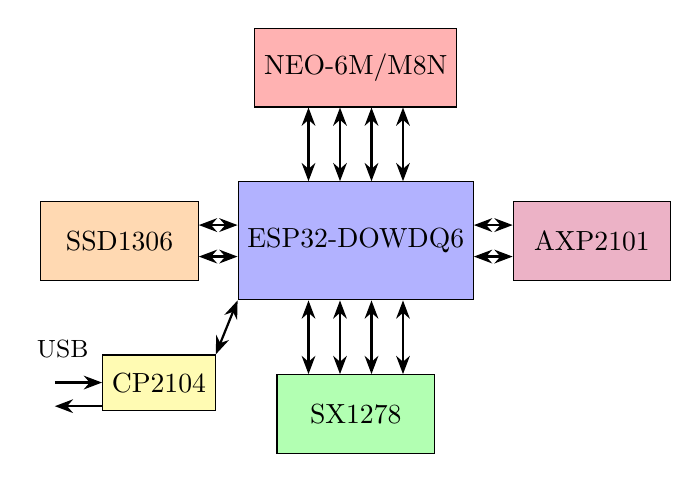
\begin{tikzpicture}[
    block/.style={rectangle, draw, text centered, minimum width=2cm, minimum height=1cm},
    arrow/.style={<->, >=Stealth, thick}
]


\coordinate (center) at (0,0);
\coordinate (top) at (0,2.2);
\coordinate (bottom) at (0,-2.2);
\coordinate (left) at (-3,0);
\coordinate (right) at (3,0);
\coordinate (diagonal) at (-2.5,-1.8);


\node[block, fill=blue!30, minimum width=2.5cm, minimum height=1.5cm] (center_block) at (center) {ESP32\\-DOWDQ6};
\node[block, fill=red!30] (top_block) at (top) {NEO-6M/M8N};
\node[block, fill=green!30] (bottom_block) at (bottom) {SX1278};
\node[block, fill=orange!30] (left_block) at (left) {SSD1306};
\node[block, fill=purple!30] (right_block) at (right) {AXP2101};
\node[block, fill=yellow!30, minimum width=1.2cm, minimum height=0.7cm] (diagonal_block) at (diagonal) {CP2104};


\draw[arrow] ([xshift=-6mm]center_block.north) -- ([xshift=-6mm]top_block.south);
\draw[arrow] ([xshift=-2mm]center_block.north) -- ([xshift=-2mm]top_block.south);
\draw[arrow] ([xshift=2mm]center_block.north) -- ([xshift=2mm]top_block.south);
\draw[arrow] ([xshift=6mm]center_block.north) -- ([xshift=6mm]top_block.south);


\draw[arrow] ([xshift=-6mm]center_block.south) -- ([xshift=-6mm]bottom_block.north);
\draw[arrow] ([xshift=-2mm]center_block.south) -- ([xshift=-2mm]bottom_block.north);
\draw[arrow] ([xshift=2mm]center_block.south) -- ([xshift=2mm]bottom_block.north);
\draw[arrow] ([xshift=6mm]center_block.south) -- ([xshift=6mm]bottom_block.north);


\draw[arrow] ([yshift=2mm]center_block.west) -- ([yshift=2mm]left_block.east);
\draw[arrow] ([yshift=-2mm]center_block.west) -- ([yshift=-2mm]left_block.east);


\draw[arrow] ([yshift=2mm]center_block.east) -- ([yshift=2mm]right_block.west);
\draw[arrow] ([yshift=-2mm]center_block.east) -- ([yshift=-2mm]right_block.west);


\draw[arrow] (center_block.south west) -- (diagonal_block.north east);

\draw[->, >=Stealth, thick] ([xshift=-6mm]diagonal_block.west) -- (diagonal_block.west);
\draw[<-, >=Stealth, thick] ([xshift=-6mm, yshift=-3mm]diagonal_block.west) -- ([yshift=-3mm]diagonal_block.west);
\node[above, font=\small] at ([xshift=-5mm, yshift=2mm]diagonal_block.west) {USB};

\end{tikzpicture}
\caption{Diagrama de bloques de la placa de desarrollo \textit{LilyGo T-Beam v1.2}.}
\label{fig:diagrama-bloques}
\end{figure}

\section{Diseño de la solución}

La propuesta busca resolver un problema común en fincas medianas y grandes, localizar animales de granja y animales domésticos. Para ello, se plantea colocar collares no invasivos a los animales, que contengan un dispositivo con una carcasa protectora contra factores mecánicos y ambientales, para que transmitan información de localización de manera inalámbrica hacia una estación central. La comunicación se realiza con enlaces de largo alcance mediante LoRa, encapsulando los datos con el protocolo APRS, lo que permite cubrir áreas grandes con bajo consumo.

Desde la experiencia del usuario el flujo es directo: el collar toma lecturas periódicas de posición, un microcontrolador local las valida y empaqueta, y el radio envía los datos hacia un gateway ubicado en la propiedad o en un sitio elevado. El gateway recibe, decodifica y reenvía al servidor, donde se almacenan y muestran en un mapa con historiales y zonas de actividad.

El diseño contempla situaciones límite que pueden afectar la operación: pérdida de energía por batería descargada; lecturas degradadas por vegetación densa o cañones; clima adverso (lluvia, barro, polvo, altas temperaturas) que exige carcasas selladas (con antena expuesta); y degradación del enlace LoRa por distancia o interferencias. Para mitigar, el sistema reintenta envíos y mantiene colas locales para subidas diferidas cuando vuelve la cobertura, es responsabilidad del usuario el control de energía de cada dispositivo.

En su versión final, el producto se visualiza como una red de collares autónomos distribuidos en el terreno, con un microcontrolador de muy bajo consumo, radio LoRa y una posible carga solar para aumentar la autonomía del dispositivo, todo en una carcasa IP resistente. La estación central un gateway con conexión a internet o con sincronización periódica concentra la información y ofrece una interfaz para monitoreo en tiempo real, búsqueda rápida, análisis de hábitos y rutas, y gestión de grupos. Con esto se mejora la seguridad (detección temprana de escapes o robo de animales), se ahorra tiempo en localización, y se obtiene inteligencia práctica para la administración de potreros. En la Fig \ref{fig:collar.png} se muestra un posible diseño como aplicación final del proyecto.


\begin{figure}[htbp]
    \centering
    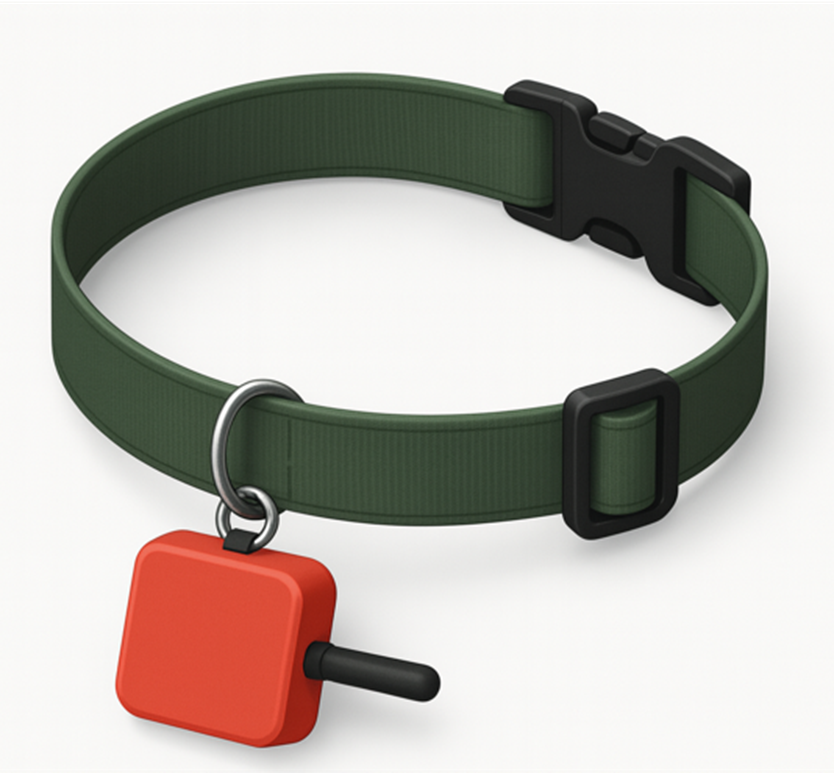
\includegraphics[width=1\linewidth]{fig/collar.png}
    \caption{Propuesta de diseño de la aplicación del proyecto}
    \label{fig:collar.png}
\end{figure}

\section{Diseño modular}

El diagrama de primer nivel expone la motivación del proyecto. El problema a resolver es el monitoreo y la localización del ganado, es decir, conocer la posición de cada animal y su dinámica de movimiento, junto con la necesidad de conexión en zonas remotas donde no siempre hay cobertura celular. La solución propuesta es un esquema de monitoreo mediante LoRa y APRS. El dispositivo obtiene posición y estado, los empaqueta en tramas ligeras y los transmite por radio a larga distancia. A partir de este proceso se obtienen dos salidas: datos de posición geográfica (ubicación actual de cada animal) e información histórica (trayectorias, permanencias, entradas y salidas de geocercas, e inactividad). Estos datos permiten alcanzar el resultado buscado: mejora en el control de grupos, habilitando decisiones de manejo como reunir, mover, o detectar fuga y rezago.

\begin{figure}[htbp]
    \centering
    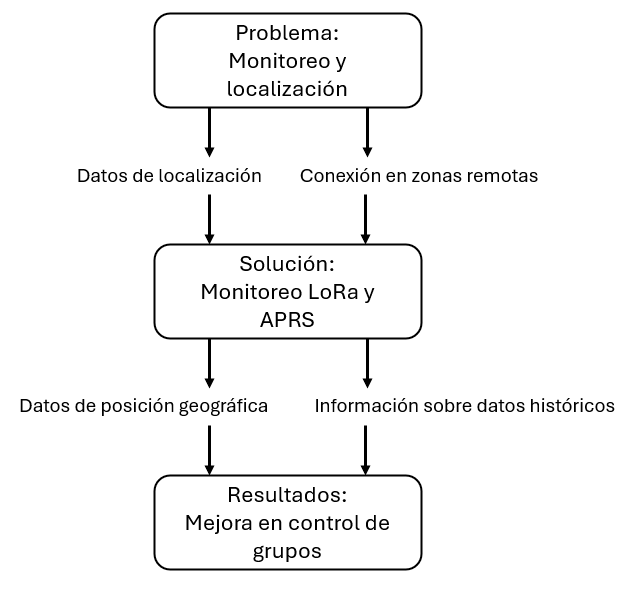
\includegraphics[width=0.9\linewidth]{fig/primer_nivel.png}
    \caption{Diagrama de primer nivel del sistema}
    \label{fig:primer_nivel}
\end{figure}

El diagrama de segundo nivel describe los roles del sistema y el flujo de información.

\begin{itemize}
    \item \textbf{Solución: Monitoreo LoRa y APRS.} Representa el conjunto collar y radio, que toma mediciones locales (posición, batería, movimiento) y emite tramas por el enlace LoRa/APRS.
    \item \textbf{GPS.} Módulo que entrega datos de posición geográfica al dispositivo. El tracker lee estas tramas (NMEA o binario) y decide si reporta de inmediato o conserva la información hasta el siguiente intervalo.
    \item \textbf{Gateway central.} Equipo fijo que recibe las tramas por radio, las decodifica (parámetros de radio y formato del \emph{payload}) y publica eventos hacia el \emph{backend}. La flecha de solicitud de datos indica que desde el \emph{backend} se pueden enviar \emph{downlinks} (por ejemplo, cambio de intervalo o habilitación de búsqueda) que el gateway reinyecta al aire.
    \item \textbf{Interfaz del usuario.} Panel web o aplicación que recibe datos procesados (posiciones ya interpretadas con reglas de negocio) y puede originar peticiones o comandos de configuración que regresan al gateway como \emph{downlinks}.
\end{itemize}

\begin{figure}[htbp]
    \centering
    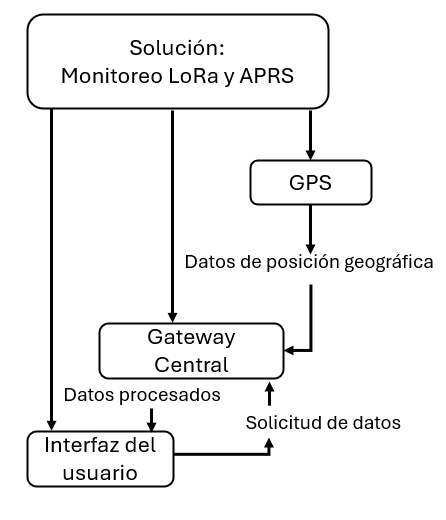
\includegraphics[width=0.9\linewidth]{fig/segundo_nivel.png}
    \caption{Diagrama de segundo nivel del sistema}
    \label{fig:segundo_nivel}
\end{figure}

El diagrama de tercer nivel elimina la caja negra y muestra componentes internos y su interacción.

\begin{itemize}
    \item \textbf{GPS a Microcontrolador.} El receptor entrega posición, tiempo y calidad del \emph{fix}. El microcontrolador (por ejemplo, ESP32/T-Beam) filtra y valida: si el \emph{fix} es válido y coincide con una ventana de reporte, empaqueta la ubicación.
    \item \textbf{PMIC a Microcontrolador (energía) y Microcontrolador a PMIC (control).} El PMIC suministra 3{,}3~V y gestiona batería y carga. A su vez, el microcontrolador ordena encender o apagar rieles (GPS y radio) para ahorrar energía, implementando el ciclo dormir–despertar–medir–enviar.
    \item \textbf{Microcontrolador a Módulo LoRa.} El microcontrolador envía el dato procesado (payload compacto) por SPI al transceptor. El radio modula y transmite por la antena. Cuando corresponde, abre ventanas de recepción para \emph{downlinks}.
    \item \textbf{Módulo LoRa a Gateway central.} El gateway recibe la trama aérea y la entrega al servidor de red, donde se decodifica (llaves, puerto y esquema del \emph{payload}) y se normaliza.
    \item \textbf{Gateway central a Base de datos.} Una vez decodificados, los datos se almacenan (latitud, longitud, batería, RSSI/SNR y marcas de tiempo). Con estos registros se calculan métricas e historiales.
    \item \textbf{Base de datos a Interfaz de usuario.} La aplicación consulta y muestra capas útiles: mapa en vivo, geocercas, alertas (salida de potrero e inactividad), estado de batería y cobertura. Desde la interfaz también se generan órdenes que regresan como \emph{downlinks} al dispositivo (correspondientes a la solicitud de datos del nivel 2).
\end{itemize}

\begin{figure}[htbp]
    \centering
    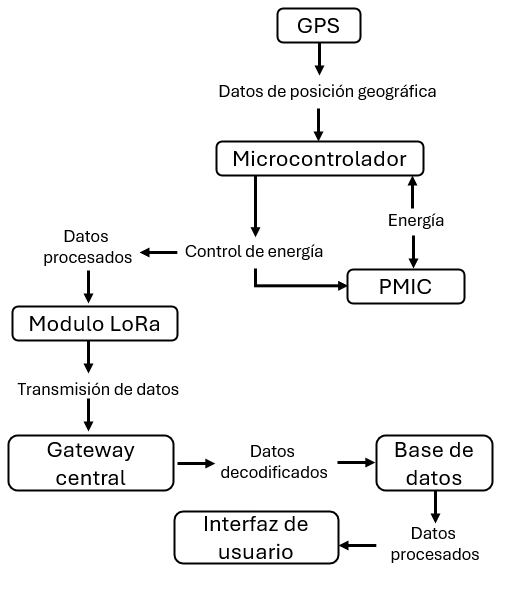
\includegraphics[width=0.9\linewidth]{fig/tercer_nivel.png}
    \caption{Diagrama de tercer nivel del sistema}
    \label{fig:tercer_nivel}
\end{figure}

\section{Características avanzadas del sistema}

El sistema propuesto no se limita a transmitir coordenadas de posición, sino que incorpora una serie de características avanzadas que lo diferencian de un tracker básico y lo orientan a una aplicación productiva en fincas medianas y grandes.

El diseño integra una gestión avanzada de energía mediante el PMIC AXP2101 y las capacidades de bajo consumo del ESP32-DOWDQ6. El microcontrolador puede controlar la alimentación de los módulos GPS y LoRa, habilitándolos únicamente durante ventanas de medición y transmisión. Esto permite maximizar la autonomía en campo y hacer viable el uso del dispositivo en collares alimentados por baterías recargables, e incluso considerar la integración futura de carga solar.

Además, el sistema hace uso combinado de LoRa y APRS. LoRa proporciona el enlace de largo alcance y baja potencia, mientras que APRS aporta una estructura estándar de tramas pensada para telemetría y localización, lo que permite aprovechar infraestructura ya existente (IGates) y al mismo tiempo mantener flexibilidad para definir diferentes tipos de beacons y cargas útiles según la necesidad de la aplicación (solo posición, posición con nivel de batería, estados especiales, entre otros).

A nivel de arquitectura de software, el firmware integra módulos reutilizables provenientes de librerías de código abierto, lo que facilita añadir funcionalidades avanzadas, como la configuración remota de parámetros (intervalo de reporte, modos de búsqueda, niveles de potencia de transmisión) por medio de downlinks desde el gateway, la definición de políticas de reporte, en las que el tracker puede modificar su frecuencia de transmisión según el movimiento del animal, el nivel de batería o la calidad del enlace. Integración con servicios web y bases de datos que permiten generar historiales, geocercas, alertas de salida de potrero y análisis de rutas.

El tracker incorpora el uso de smartbeaconing y el envío de una trama institucional con telemetría integrada. El smartbeaconing permite ajustar de forma automática el intervalo de transmisión de beacons según el movimiento del tracker: cuando el animal está prácticamente en reposo, el dispositivo envía tramas con menor frecuencia para ahorrar batería y reducir la ocupación del canal; a medida que aumenta la velocidad o se detectan cambios significativos de rumbo, la frecuencia de reporte se incrementa para capturar mejor la trayectoria. Paralelamente, la trama institucional asegura que cada transmisión incluya la identificación del proyecto y la información relevante para el sistema de monitoreo, incorporando campos de telemetría como el voltaje de la batería sin requerir modificaciones profundas al firmware.

Por último, el sistema contempla desde su diseño la escalabilidad y la interoperabilidad. El uso de protocolos establecidos (UART para GPS, SPI para LoRa, I²C para la OLED y sensores auxiliares) permite integrar otros dispositivos en el futuro, como sensores de actividad, temperatura o salud del animal, sin alterar la arquitectura base. Del lado del backend, la utilización de tramas normalizadas y almacenamiento estructurado de la información facilita la integración con aplicaciones web de terceros, paneles de visualización y herramientas analíticas orientadas a la toma de decisiones en manejo de ganado.

\section{Diagrama eléctrico}

Para el sistema utilizado se presenta el diagrama eléctrico de la tarjeta de desarrollo del tracker, el ESP32 del LilyGo's T-Beam ESP32 LoRa 433MHz SX1276 \cite{tbeam_v12_schematic}. El ESP32 gobierna la radio LoRa mediante el bus SPI y líneas adicionales de control. El SPI suministra reloj, datos y selección de chip al transceptor, mientras un par de GPIO se asignan a las interrupciones del radio y a la señal de reinicio. Esta arquitectura permite operar el firmware en Clase A: el radio permanece en reposo la mayor parte del tiempo, se activa para transmitir la trama de posición y vuelve al modo de bajo consumo cuando finalizan las ventanas de recepción. El enlace de RF sale de la placa a través de un conector de antena y una pista de 50 ohm, lo que permite ubicar la antena en el exterior de la caja roja del collar para maximizar la cobertura en campo.

El GPS se conecta al ESP32 por un puerto UART dedicado. El par TX/RX se utiliza para configurar el receptor y para leer tramas NMEA o formato binario, y se puede emplear la salida de pulso por segundo para estampar tiempo con precisión cuando sea necesario. La alimentación del GPS se gestiona desde el microcontrolador mediante una línea de habilitación o un riel conmutable del gestor de energía, de modo que el receptor permanezca apagado entre mediciones y solo se energice durante una ventana breve para obtener el arreglo y conservar efemérides, con la consiguiente reducción del tiempo a primer arreglo y del consumo total.

La alimentación del T-Beam parte de una celda de ion litio o polímero de litio y entra a un PMIC con cargador integrado. Este gestor entrega un riel principal a 3,3 V para el ESP32 y, según el diseño de la placa, rieles conmutables para el módulo LoRa y el GPS. Desde la perspectiva del diagrama, el microcontrolador controla estos rieles mediante pines de habilitación, lo que proporciona un control de energía a nivel de hardware y posibilita autonomías prolongadas en campo. El puerto USB con su convertidor USB a UART se reserva para programación y diagnóstico en taller, y el mismo conector alimenta al PMIC para la recarga de la batería antes de sellar la caja.

Finalmente, conviene destacar dos aspectos eléctricos clave para esta aplicación rural: la ruta de RF hasta el conector de antena, incluida la red de adaptación, ya que la antena se instalará en el exterior o en una zona del encapsulado con buena transparencia electromagnética, y la separación lógica de buses, con SPI para la radio, UART para el GPS e I²C para sensores auxiliares como la IMU o el medidor de batería. 

\begin{figure}[htbp]
    \centering
    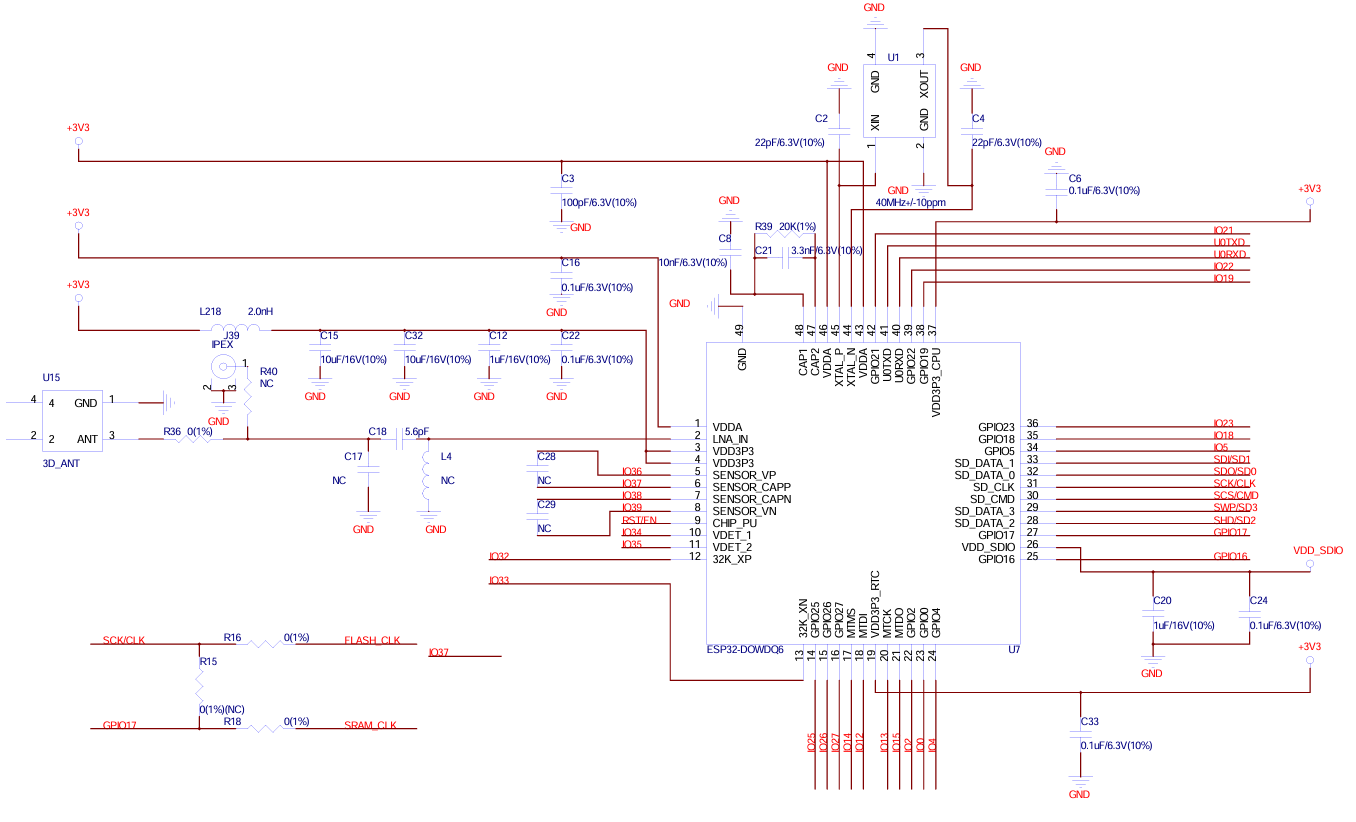
\includegraphics[width=0.9\linewidth]{fig/electrico.png}
    \caption{Diagrama eléctrico interno del ESP32 \cite{tbeam_v12_schematic}}
    \label{fig:electrico}
\end{figure}

\section{Tipo de comunicación de periféricos}

Los periféricos integrados en la placa de desarrollo \textit{LilyGo TTGO T-Beam v1.2} utilizan diferentes protocolos de comunicación para interactuar con el microcontrolador ESP32-DOWDQ6, los principales siendo \textit{I2C}, \textit{SPI} y \textit{UART}. Las tramas de datos son definidas acorde a las características de cada módulo, sus registros propios y las capacidades de cada uno. Para el caso particular del transceptor LoRa SX1278, se utiliza el protocolo SPI para la comunicación con el microcontrolador, permitiendo la configuración de parámetros como frecuencia, potencia de transmisión, ancho de banda y demás ajustes necesarios para la operación del módulo. La comunicación con el receptor GPS NEO-6M/M8N se realiza a través del protocolo UART, enviando y recibiendo datos en formato NMEA que contienen información de posición, velocidad y tiempo. La pantalla OLED SSD1306 utiliza el protocolo I2C para recibir comandos e información gráfica desde el microcontrolador, permitiendo la visualización de datos en tiempo real.

\begin{figure}[h!]
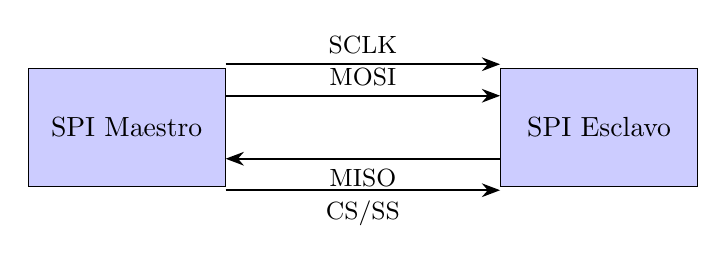
\begin{tikzpicture}[
    block/.style={rectangle, draw, fill=blue!20, text centered, minimum width=2.5cm, minimum height=1.5cm},
    arrow/.style={->, >=Stealth, thick},
    signal/.style={font=\small}
]

\node[block] (master) at (0,0) {SPI Maestro};
\node[block] (slave) at (6,0) {SPI Esclavo};

\draw[arrow] ([yshift=8mm]master.east) -- ([yshift=8mm]slave.west) node[midway, above, signal] {SCLK};
\draw[arrow] ([yshift=4mm]master.east) -- ([yshift=4mm]slave.west) node[midway, above, signal] {MOSI};
\draw[arrow] ([yshift=-4mm]slave.west) -- ([yshift=-4mm]master.east) node[midway, below, signal] {MISO};
\draw[arrow] ([yshift=-8mm]master.east) -- ([yshift=-8mm]slave.west) node[midway, below, signal] {CS/SS};

\end{tikzpicture}
\caption{Diagrama de comunicación SPI.}
\end{figure}
\vspace{2cm}
\begin{figure}[h!]
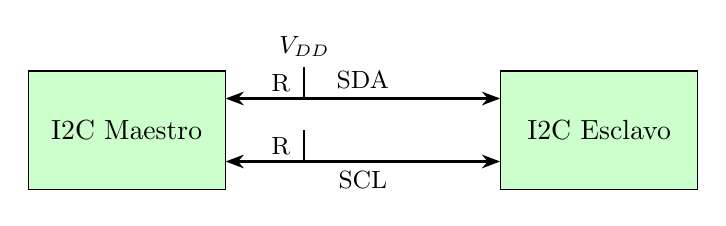
\begin{tikzpicture}[
    block/.style={rectangle, draw, fill=green!20, text centered, minimum width=2.5cm, minimum height=1.5cm},
    arrow/.style={<->, >=Stealth, thick},
    signal/.style={font=\small}
]

\node[block] (master) at (0,0) {I2C Maestro};
\node[block] (slave) at (6,0) {I2C Esclavo};

\draw[arrow] ([yshift=4mm]master.east) -- ([yshift=4mm]slave.west) node[midway, above, signal] {SDA};
\draw[arrow] ([yshift=-4mm]master.east) -- ([yshift=-4mm]slave.west) node[midway, below, signal] {SCL};

\draw[thick] ([xshift=1cm, yshift=4mm]master.east) -- ([xshift=1cm, yshift=8mm]master.east) node[above, signal] {$V_{DD}$};
\draw[thick] ([xshift=1cm, yshift=-4mm]master.east) -- ([xshift=1cm, yshift=0mm]master.east);
\node[signal] at ([xshift=0.7cm, yshift=6mm]master.east) {R};
\node[signal] at ([xshift=0.7cm, yshift=-2mm]master.east) {R};

\end{tikzpicture}
\caption{Diagrama de comunicación I2C.
\label{fig:i2c}}
\end{figure}

\begin{figure}[h!]
    \centering
    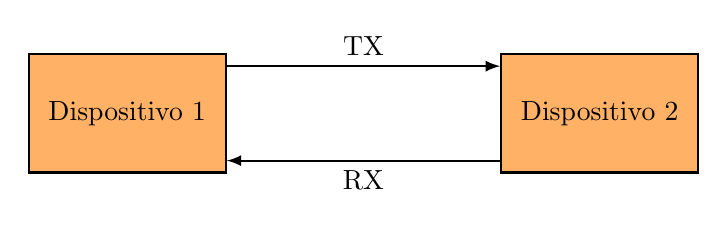
\begin{tikzpicture}[>=latex, thick]

        \coordinate (A) at (0,0);
        \coordinate (B) at (6,0);

        \node[draw, fill=orange!60, minimum width=2.5cm, minimum height=1.5cm, anchor=center] (devA) at (A) {Dispositivo 1};
        \node[draw, fill=orange!60, minimum width=2.5cm, minimum height=1.5cm, anchor=center] (devB) at (B) {Dispositivo 2};

        \draw[->, black] ([yshift=0.6cm]devA.east) -- ([yshift=0.6cm]devB.west)
            node[midway, above, black] {TX};

        \draw[->, black] ([yshift=-0.6cm]devB.west) -- ([yshift=-0.6cm]devA.east)
            node[midway, below, black] {RX};

    \end{tikzpicture}
    \caption{Diagrama de comunicación UART.}
    \label{fig:uart-tx-rx}
\end{figure}

Nótese que en las figura \ref{fig:i2c}, se incluyen resistencias de pull-up en las líneas de datos, las cuales son esenciales para el correcto funcionamiento del protocolo I2C, asegurando niveles lógicos adecuados y evitando estados flotantes que podrían causar errores en la comunicación, además que a diferencia de \textit{I2C} y \textit{SPI}, el protocolo \textit{UART} no requiere de una línea de reloj, ya que la sincronización se logra mediante la configuración previa de la velocidad de transmisión (baud rate) en ambos dispositivos y en vez de tener una arquitectura maestro-esclavo, ambos dispositivos pueden enviar y recibir datos de manera independiente, siendo así \textit{full-duplex}.

El resto de detalles de sobre las características eléctricas, el esquemático y los archivos \textit{CAD} de la placa de desarrollo \textit{LilyGo TTGO T-Beam v1.2} pueden ser encontrados en el repositorio oficial de \textit{GitHub} de \textit{LilyGo} que se encuentra en anexos.

\section{Pseudo-código del sistema}

Debido a que el \textit{firmware} utilizado está basado en repositorio de Ricardo Guzmán adjunto en anexos, el pseudo-código utiliza una arquitectura de \textit{superloop} propia del \textit{framework} de \textit{Arduino}, la cual es sencilla y eficiente para aplicaciones embebidas. A continuación, se presenta un diagrama simplificado que ilustra la estructura general del programa:

\begin{figure}[h!]
\begin{center}
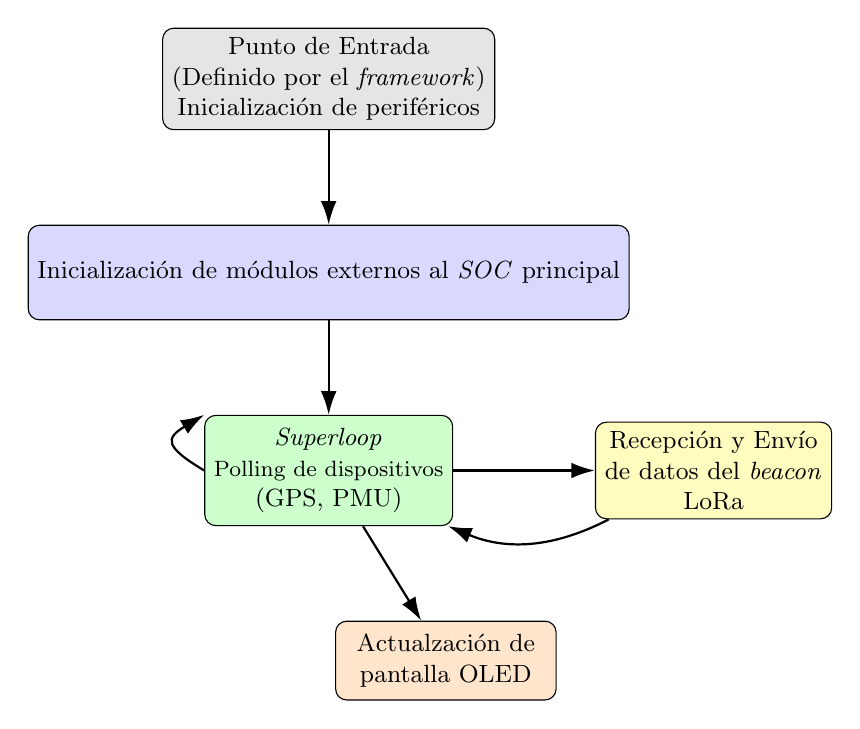
\begin{tikzpicture}[
    node distance=1.2cm and 2.5cm,
    every node/.style={rectangle, draw=black, rounded corners, align=center, font=\small},
    arrow/.style={-{Latex[length=3mm,width=2mm]}, thick}, % shorter arrows
    init/.style={fill=blue!15, minimum width=4cm, minimum height=1.2cm},
    super/.style={fill=green!20, minimum width=3cm, minimum height=1.4cm},
    idle/.style={fill=yellow!25, minimum width=3cm, minimum height=1.2cm},
    start/.style={fill=gray!20, minimum width=4cm, minimum height=1.2cm},
    display/.style={fill=orange!20, minimum width=2.8cm, minimum height=1cm}
]

\node[start] (start) {Punto de Entrada\\(Definido por el \textit{framework})\\Inicialización de periféricos};
\node[init, below=of start] (init) {Inicialización de módulos externos al \textit{SOC} principal};
\node[super, below=of init] (superloop) {\textit{Superloop}\\\footnotesize Polling de dispositivos\\(GPS, PMU)};
\node[idle, right=1.8cm of superloop] (idle) {Recepción y Envío\\ de datos del \textit{beacon}\\ LoRa};
\node[display, below right=1.2cm and -1.5cm of superloop] (display) {Actualzación de\\ pantalla OLED};

\draw[arrow] (start) -- (init);
\draw[arrow] (init) -- (superloop);
\draw[arrow] (superloop) -- (idle);
\draw[arrow] (idle) to[bend left=25] (superloop);
\draw[arrow] (superloop) -- (display);
\draw[arrow] (superloop.west) .. controls +(-0.5,0.3) and +(-0.5,-0.3) .. (superloop.north west);

\end{tikzpicture}
\end{center}
\label{fig:flujo}
\caption{Diagrama simplificado del flujo del programa.}
\end{figure}

El código utiliza \textit{APIs} públicas de proyectos de código abierto, las cuales permiten la configuración y manejo de los periféricos integrados en la placa de desarrollo, un ejemplo de esto es \textit{RadioLib} adjunto en anexos, la cual es una librería para comunicación inalámbrica que soporta múltiples módulos de radio, incluyendo LoRa, y proporciona una interfaz sencilla para configurar y utilizar el transceptor SX1278. La librería maneja detalles complejos de la comunicación LoRa, como la modulación, codificación y gestión de paquetes, permitiendo a los desarrolladores centrarse en la lógica de su aplicación sin preocuparse por los aspectos de bajo nivel del protocolo LoRa, permitiendo además la configuración de parámetros como la frecuencia, potencia de transmisión, ancho de banda y otros ajustes necesarios para la correcta operación.

De manera similar, el código provee una gran cantidad de utiliarios \textit{wrappers} de librerías de Arduino para la gestión de más recursos de la placa, un claro ejemplo de esto son las librerías \textit{web\_utils.h}, \textit{wx\_utils.h} y \textit{wifi\_utils.h}

\section{Tramas de datos utilizadas}

El tracker utiliza la estructura estándar de paquetes APRS (Automatic Packet Reporting System) para la transmisión y recepción de datos de localización y telemetría. A continuación se muestra una tabla con una trama sencilla de un paquete APRS, con un ejemplo ilustrativo:

\small

\vspace{0.5em}
\begin{figure}[h!]
\begin{tabular}{@{} l l l c l @{}}
\toprule
\textbf{Fuente} \textbf{>}& \textbf{Destino} & \textbf{,}\textbf{Camino} & \textbf{:} & \textbf{INFO}\\
\midrule
N0CALL-7 & APRS & WIDE1-1,WIDE2-1 & : & MSG! \\
\bottomrule
\end{tabular}
\caption{Estructura general de un paquete APRS.}
\label{fig:trama-aprs}
\end{figure}

Nótese que en la figura \ref{fig:trama-aprs}, el símbolo utilizado es ">", pero este y otros parámetros son configurables en el archivo \textit{tracker\_conf.json}, el cual es leído por el \textit{firmware} al momento de inicializar el sistema, además permite tener diferentes tipos de \textit{beacons}, cada uno con su configuración particular de acuerdo a las necesidad de la aplicación.
En la imagen \ref{fig:tramas-ejemplo} se presentan algunos ejemplos de tramas APRS recibidas por el \textit{tracker}.

\begin{figure}[htbp]
\begin{tabular}{|l|}
\hline
TI2BSH-7>APLRT1,TI2JR-10*:!/IN-m97CebNMQ\\
\hline
TI2BSH-10>APLRG1,TI2JR-10*:!LIN-96Q-a  GLoRa APR\\
\hline
TI2JR-10>APLRG1,WIDE1-1:!LIJgp9;"M  GLoRa APRS \\
\hline
\end{tabular}
\caption{Ejemplos de tramas APRS recibidas y transmitidas por el \textit{tracker}.}
\label{fig:tramas-ejemplo}
\end{figure}
% you can choose not to have a title for an appendix
% if you want by leaving the argument blank
\vspace{1cm}


\section{Cumplimiento de leyes y legislación}

El sistema propuesto opera en bandas de radiofrecuencia y, por tanto, se ajusta a la normativa vigente en Costa Rica y a los estándares internacionales aplicables a los servicios utilizados (APRS y LoRa).

En relación con APRS, el servicio se utiliza típicamente en la banda de VHF alrededor de 144–148 MHz, atribuida al servicio de radioaficionados. De acuerdo con el Plan Nacional de Atribución de Frecuencias (PNAF) y el Manual del Radioaficionado de SUTEL \cite{sutel_manual_radioaficionados_2014}, la operación en estas frecuencias requiere contar con una licencia vigente de radioaficionado en las categorías Novicio, Intermedio o Superior. En el contexto del proyecto, se considera que:

Las transmisiones APRS realizadas para las pruebas se efectúan bajo el indicativo y la licencia del radioaficionado responsable del experimento.
La potencia de transmisión configurada en el equipo se mantiene por debajo de los límites establecidos para la categoría de licencia utilizada.
Se respetan las recomendaciones de uso compartido del canal y la naturaleza experimental/telemetría del tráfico APRS, evitando usos que contravengan la reglamentación del servicio de aficionados \cite{micitt_pnaf_2023}.

En cuanto a LoRa, el sistema hace uso de bandas de uso libre definidas en el PNAF para aplicaciones de corto alcance, específicamente en el rango de 433,05 a 434,79 MHz y en el rango de novecientos 20,5 a 928 MHz para Costa Rica \cite{sutel_manual_radioaficionados_2014}. La normativa establece un límite de Potencia Isotrópica Radiada Equivalente (PIRE) de treinta decibelios-miliwatt para estos segmentos. El diseño del tracker cumple estos requisitos al:

\begin{itemize}

\item Seleccionar como frecuencia de operación una portadora incluida en las bandas de uso libre permitidas.

\item Configurar el transceptor LoRa con un nivel de potencia de salida y una ganancia de antena tales que la PIRE resultante no exceda el límite de treinta decibelios-miliwatt.

\item Emplear un esquema de transmisión de baja ocupación, con tramas cortas y espaciadas, minimizando la probabilidad de interferencia con otros usuarios de la banda.

\end{itemize}

Desde la perspectiva de estándares y designadores de emisión, se identificó que:

\begin{itemize}

\item APRS puede clasificarse como una emisión F1D (modulación en frecuencia, una portadora, transmisión de datos/telemetría).

\item LoRa, por su naturaleza de modulación de espectro ensanchado basada en barridos de frecuencia, puede asimilarse a una emisión G1D (modulación en fase, una portadora, transmisión de datos/telemetría).

\item El tracker se ha configurado de forma que sus parámetros de operación (ancho de banda, factor de expansión, tiempo de ocupación de canal) se mantengan dentro de lo esperable para este tipo de servicios de baja potencia y largo alcance, respetando los perfiles de emisión asociados a dichas designaciones.

\end{itemize}

Finalmente, desde el punto de vista de buenas prácticas de ingeniería, el sistema emplea módulos de radio comerciales que cumplen con certificaciones de compatibilidad electromagnética y seguridad eléctrica en los mercados donde se comercializan, y la topología propuesta para la instalación en campo (collar con antena exterior, gateway fijo y backend remoto) prioriza la operación en bandas no licenciadas y el cumplimiento de los límites de potencia. Con base en lo anterior, el sistema cumple con la normativa costarricense aplicable y se alinea con los estándares técnicos internacionalmente aceptados para aplicaciones de telemetría y rastreo de bajo consumo.

\section{Resultados}

En el dispositivo, se logró la configuración y operación del módulo LilyGo T-Beam v1.2 como tracker LoRa/APRS. El firmware permite obtener lecturas de posición a partir del receptor GPS, empaquetarlas en tramas APRS y transmitirlas a través del transceptor LoRa. Como resultado visible para el usuario, se actualizó el recurso gráfico desplegado en la pantalla OLED, sustituyendo el ícono genérico por uno asociado semánticamente a la aplicación de rastreo ganadero. Esta mejora, aunque es sencilla, contribuye a una interfaz más intuitiva y orientada al caso de uso final.

\begin{figure}[htbp]
    \centering
    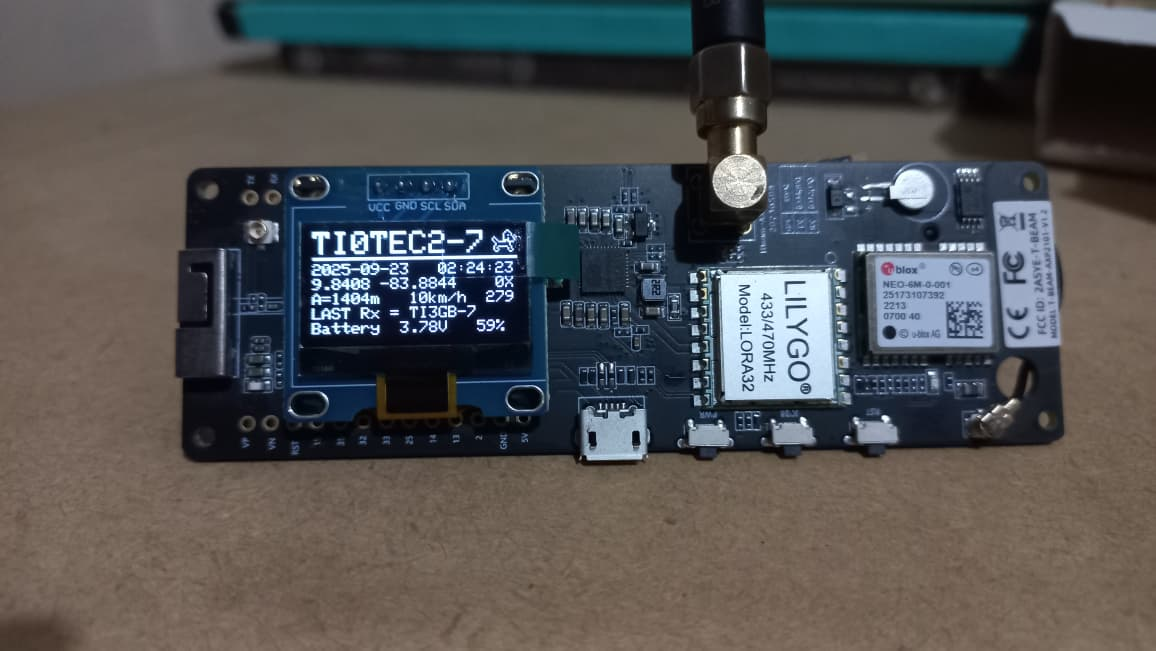
\includegraphics[width=1\linewidth]{fig/preeliminares.jpg}
    \caption{Presentación en el tracker de resultados preeliminares}
    \label{fig:preeliminares.jpg}
\end{figure}

Además, fue posible visualizar el tracker en el mapa de APRS Track Direct, se puede observar parte de un recorrido simple realizado en el campus central de Tecnológico de Costa Rica, se puede denotar tambien la utilización de un animal como simbolo para el tracker, con el fin de hacer alusión a la aplicación desarrollada.

\begin{figure}[htbp]
    \centering
    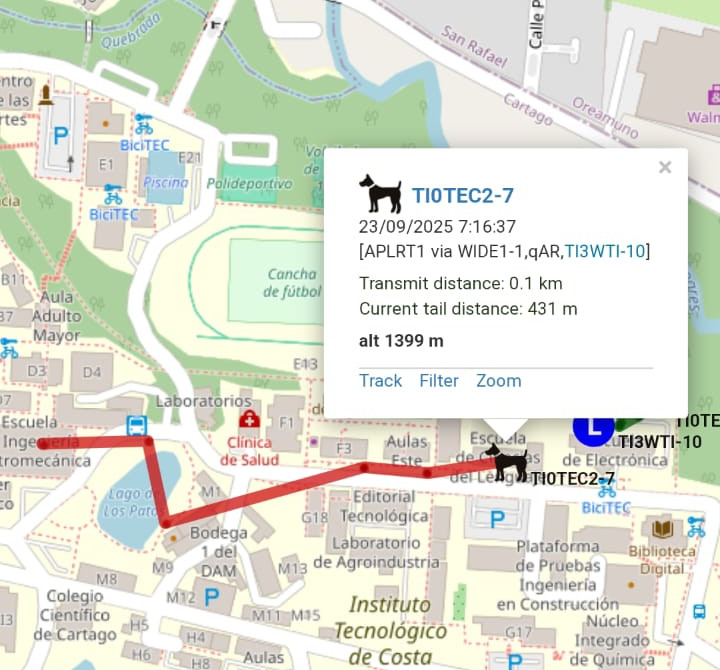
\includegraphics[width=1\linewidth]{fig/resultado-tracker.jpeg}
    \caption{Vista del tracker en el mapa de APRS Track Direct}
    \label{fig:track-direct1.jpg}
\end{figure}

Adicionalmente, se implementó una política de ahorro energético en la pantalla, de modo que el display se mantiene encendido únicamente durante un intervalo breve tras el encendido o después de la interacción del usuario con el botón central. Transcurrido un tiempo configurado, la OLED se apaga automáticamente, reduciendo el consumo sin sacrificar la funcionalidad de monitoreo local.

Desde el punto de vista de comunicaciones, el tracker fue visualizado correctamente en el mapa de APRS Track Direct, empleando un símbolo de animal para representar el nodo en el entorno gráfico. Se realizaron recorridos de prueba en el campus del Tecnológico de Costa Rica, durante los cuales se observaron reportes periódicos de posición y se confirmó la correcta decodificación de las tramas APRS en el backend. Estos ensayos demuestran que:

\begin{itemize}

\item El formato de las tramas generadas es compatible con la infraestructura APRS existente.

\item El enlace LoRa/APRS es capaz de transportar la información de ubicación desde el tracker hasta el servidor.

\item La información resulta interpretable en una interfaz cartográfica estándar, lo que facilita su uso por parte de usuarios no técnicos.

\end{itemize}

Durante las pruebas finales se comprobó que la configuración por defecto del firmware ya permite el envío de una trama institucional junto con telemetría básica, incluyendo el valor del voltaje de la batería. 

\begin{figure}[htbp]
    \centering
    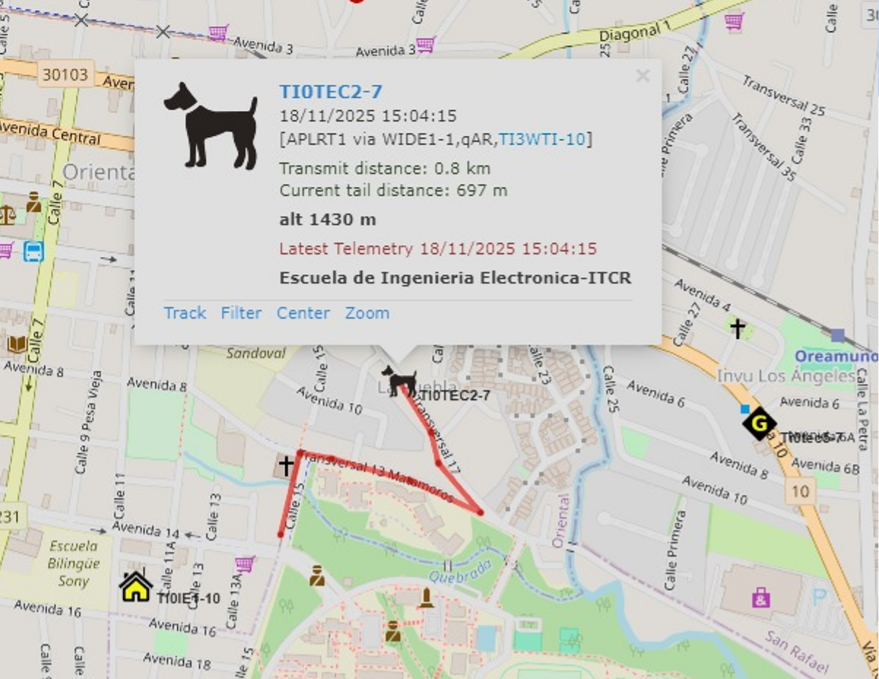
\includegraphics[width=1\linewidth]{fig/inst.png}
    \caption{Trama institucional del modulo tracker}
    \label{fig:inst.png}
\end{figure}

Esto se logra únicamente mediante los parámetros de configuración disponibles en el propio tracker. Adicionalmente, se verificó que el menú de configuración del dispositivo puede adaptarse con facilidad al idioma español, de modo que se pueda ofrecer una interfaz más amigable para el usuario final sin afectar la lógica de operación del sistema.

\begin{figure}[htbp]
    \centering
    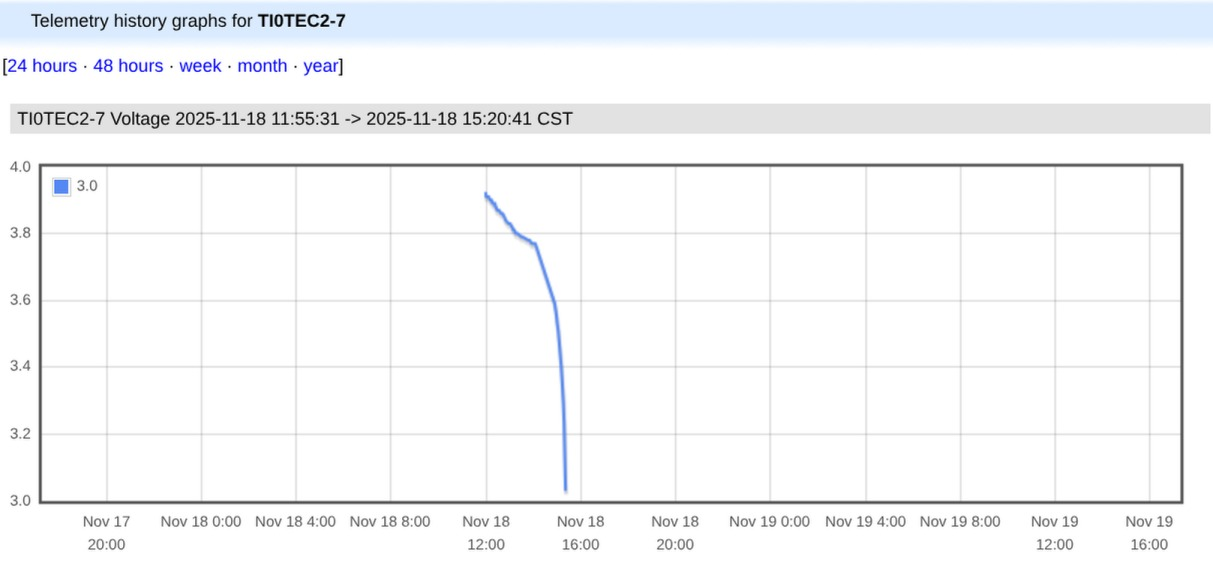
\includegraphics[width=1\linewidth]{fig/graf.jpeg}
    \caption{Desempeño de la batería en el tiempo del modulo tracker}
    \label{fig:graf.jpeg}
\end{figure}

En cuanto al comportamiento dinámico de las transmisiones, se identificó que el mecanismo de smartbeaconing se encuentra habilitado en el firmware utilizado. Este esquema ajusta el intervalo de envío de beacons en función del movimiento del tracker, incrementando la frecuencia de reporte cuando la velocidad es mayor. Durante la configuración se observó la importancia de revisar el parámetro smartBeaconSetting para cada uno de los perfiles de beacon definidos, dado que algunos perfiles lo tienen activado y otros no. Como resultado de esta revisión se estableció la necesidad de documentar claramente qué perfiles se emplearán en pruebas a pie, en vehículo u otros escenarios, y con qué ajustes de smartbeaconing asociados.

\begin{figure}[htbp]
    \centering
    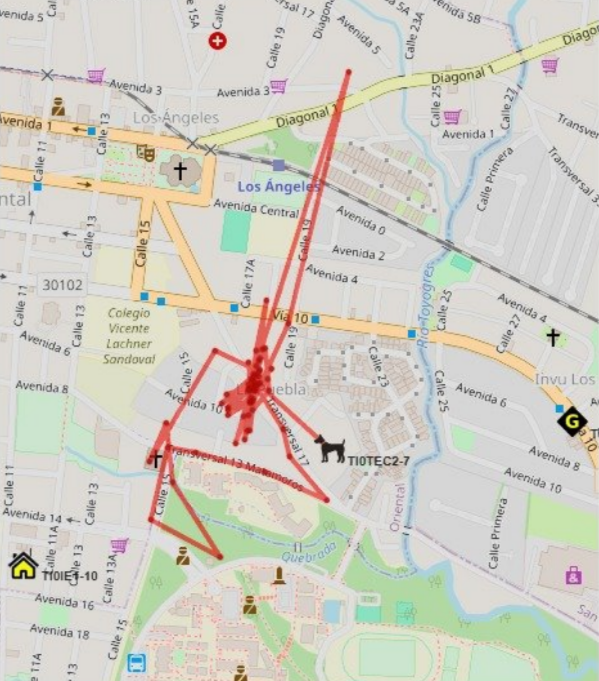
\includegraphics[width=1\linewidth]{fig/smart.png}
    \caption{Prueba de smartbeaconing del modulo tracker}
    \label{fig:smart.png}
\end{figure}

Finalmente, se realizaron ensayos de campo específicos para evaluar el comportamiento del smartbeaconing con telemetría de voltaje de batería activa. En estas pruebas el tracker se configuró para reportar tanto la posición como el nivel de batería, y se observó que, en condiciones de reposo, el intervalo entre beacons fue del orden de cuatro minutos, mientras que en movimiento se redujo aproximadamente a un rango entre un minuto y medio y dos minutos. No obstante, también se detectó que el cálculo de velocidad basado en las lecturas GPS puede presentar saltos bruscos de posición, lo cual introduce cierta imprecisión en la lógica que decide cuándo aumentar la frecuencia de transmisión. A continuación, se muestra una comparación de perfiles basado en pruebas con el tracker, que muestra los intervalos de transmisión según a la velocidad utilizando una ecuación de interpolación:

\begin{figure}[htbp]
    \centering
    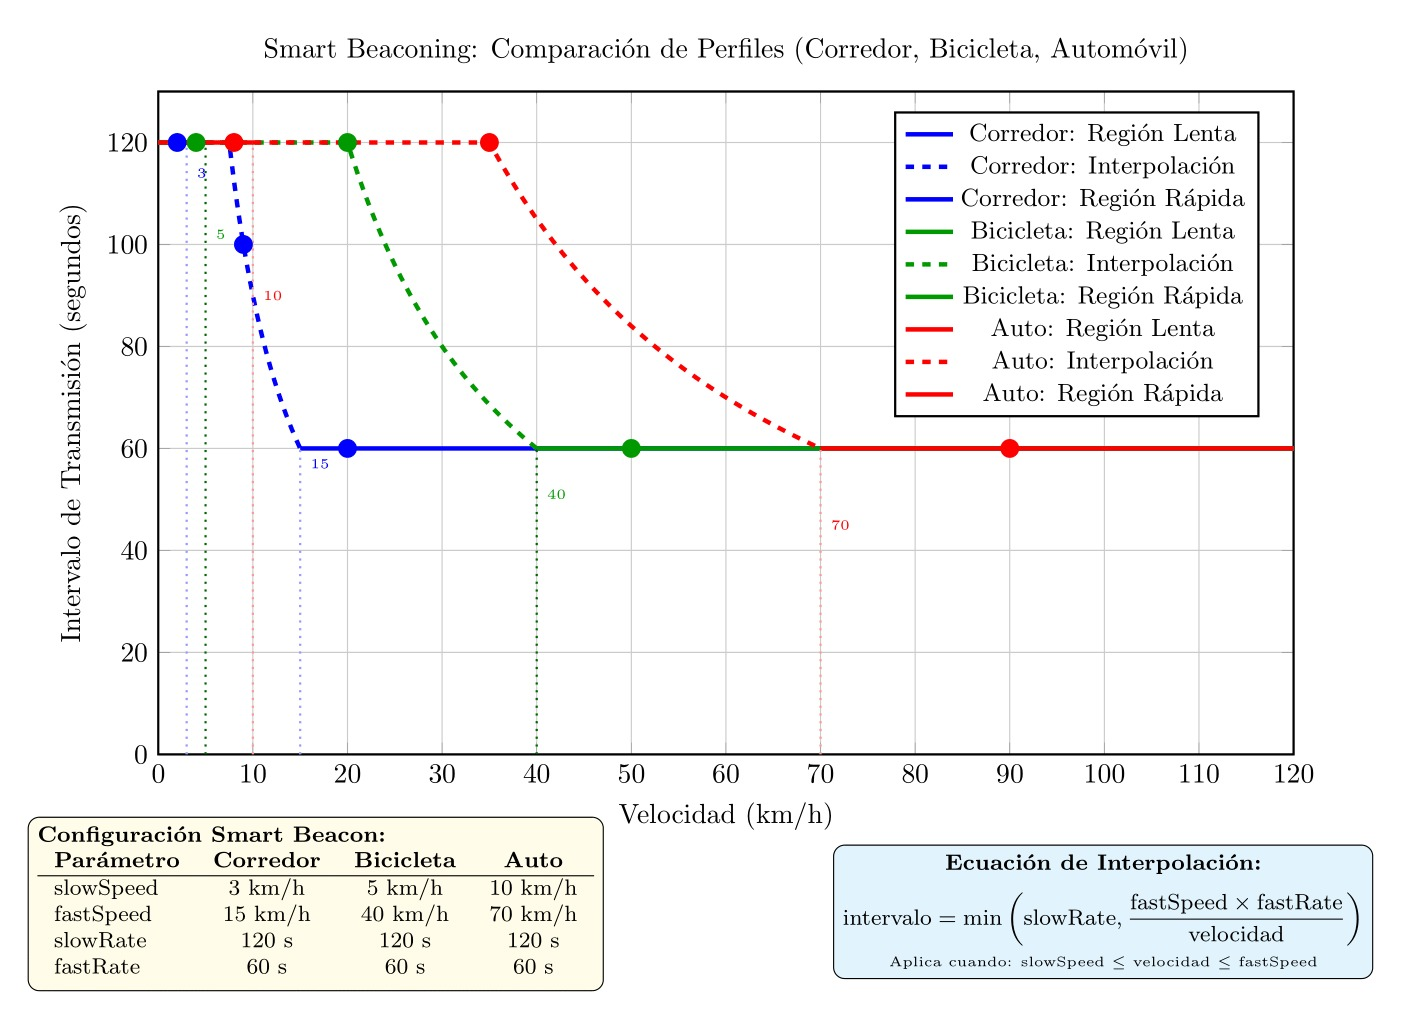
\includegraphics[width=1\linewidth]{fig/smartbeaconing.jpeg}
    \caption{Comparación de perfiles usando smartbeaconing con el modulo tracker}
    \label{fig:smartbeaconing.jpeg}
\end{figure}

\section{Presupuesto}

A continuación se muestra la Tabla \ref{tab:presupuesto} de presupuesto del proyecto, nótese que es necesario, además del módulo y su alimentación mediante una batería de Li-Ion, un collar ajustable para poner al animal, así como un protector para contener el módulo y evitar fallos por factores mecánicos y ambientales. Para un producto, se necesita una única unidad de cada elemento para su producción.

\begin{table}[!ht]
    \centering
    \small
    \renewcommand{\arraystretch}{1.3}% 
    \caption{Presupuesto estimado por unidad del tracker LoRa/APRS}
    \label{tab:presupuesto}
    \begin{tabularx}{\columnwidth}{
        >{\raggedright\arraybackslash}X
        >{\centering\arraybackslash}p{0.12\columnwidth}
        >{\centering\arraybackslash}p{0.18\columnwidth}
        >{\centering\arraybackslash}p{0.18\columnwidth}
    }
        \hline
        \textbf{Concepto} & \textbf{Cantidad} & \textbf{C. unitario [CRC]} & \textbf{C. total [CRC]} \\
        \hline
        LilyGo T-Beam v1.2 (tracker LoRa/APRS)      & 1  & 15\,500  & 15\,500  \\
        Batería Li-Ion 18650 3000 mAh               & 1  & 4\,000   & 4\,000   \\
        Collar ajustable para ganado                & 1  & 5\,000   & 5\,000   \\
        Caja / protector IP65 para módulo           & 1  & 6\,000   & 6\,000   \\
        Cables, conectores y accesorios menores     & 1  & 2\,500   & 2\,500   \\
        Impresión 3D de piezas de montaje           & 1  & 5\,000   & 5\,000   \\
        \hline
        \textbf{Subtotal hardware}                  &    &          & 38\,000  \\
        \hline
        Horas ingeniero (diseño hw/fw y pruebas)    & 20 & 37\,700  & 754\,000 \\
        \textbf{Subtotal mano de obra profesional}  &    &          & 754\,000 \\
        \hline
        Costos administrativos y varios (10\%)      &    &          & 79\,200  \\
        \hline
        \textbf{Total estimado}                     &    &          & \textbf{871\,200} \\
        \hline
    \end{tabularx}
\end{table}





\section{Cronograma}

Acorde a los avances realizados en el proyecto y los resultados obtenidos, se están cumpliendo los tiempos establecidos, por lo que se plantea continuar con el cronograma propuesto inicialmente. A continuación, se presenta el cronograma detallado de las actividades planificadas para la culminación del proyecto:

\begin{figure}[htbp]
    \centering
    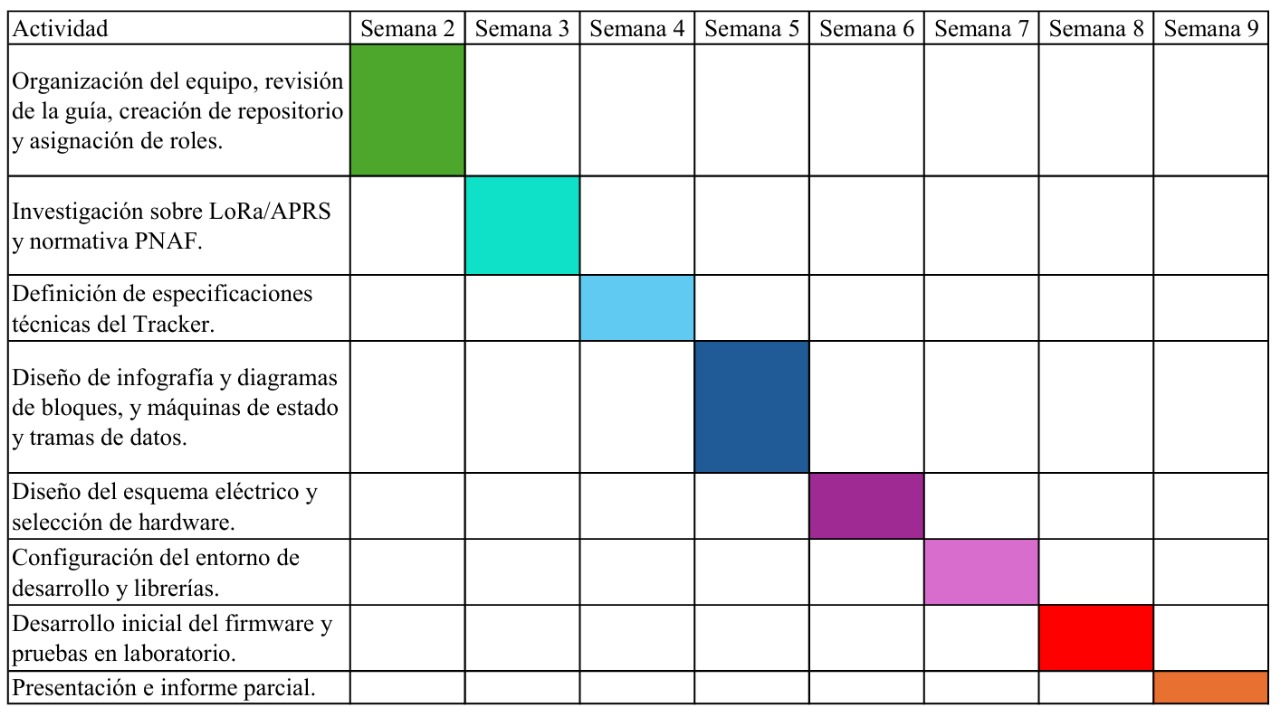
\includegraphics[width=0.9\linewidth]{fig/Gantt-1.jpeg}
    \caption{Primera Parte del Cronograma}
    \label{fig:gantt1}
\end{figure}

\begin{figure}[htbp]
    \centering
    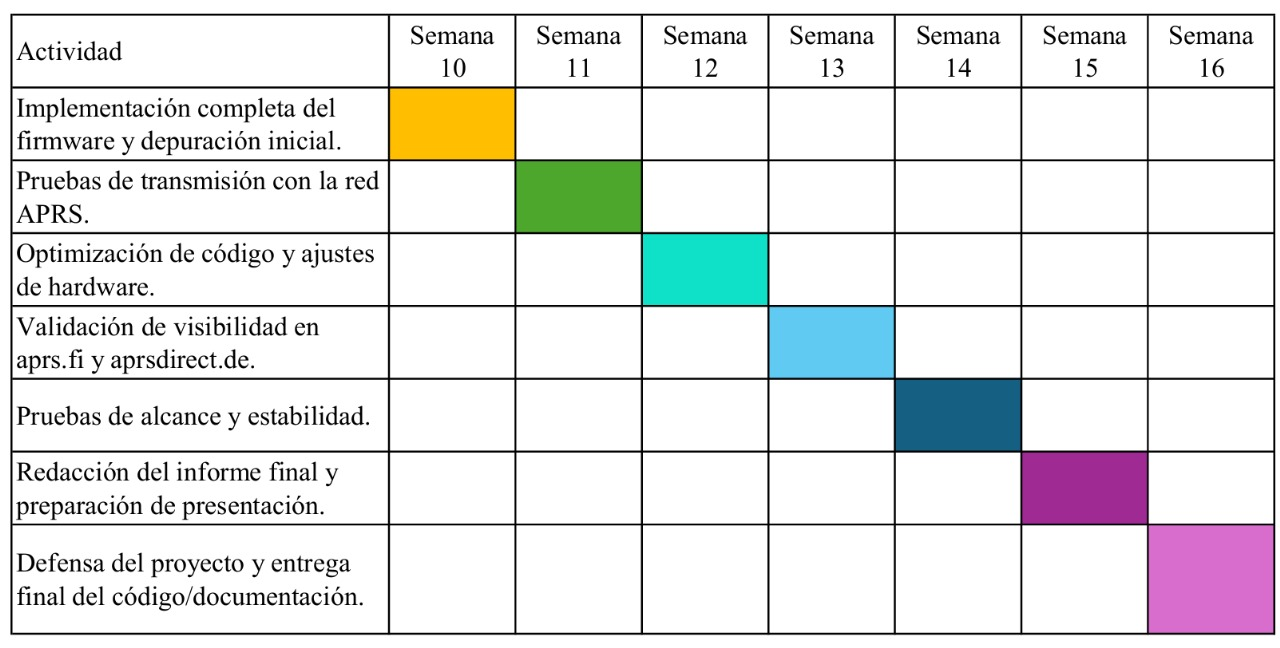
\includegraphics[width=0.9\linewidth]{fig/Gantt-2.jpeg}
    \caption{Segunda Parte del Cronograma}
    \label{fig:gantt2}
\end{figure}

\printbibliography

\section{Anexos}

\begin{itemize}
    \item \textbf{Repositorio oficial de LilyGo:} \url{https://github.com/Xinyuan-LilyGO/LilyGo-LoRa-Series}
    \item \textbf{Repositorio de Ricardo Guzmán LoRa\_APRS\_Tracker:} \url{https://github.com/richonguzman/LoRa_APRS_Tracker}
    \item \textbf{Repositorio de RadioLib:} \url{https://github.com/jgromes/RadioLib}

    \item \textbf{Repositorio del proyecto:} \url{https://github.com/NagelMS/proyecto-taller-integrador.git}
\end{itemize}



% Can use something like this to put references on a page
% by themselves when using endfloat and the captionsoff option.
\ifCLASSOPTIONcaptionsoff
  \newpage
\fi



% trigger a \newpage just before the given reference
% number - used to balance the columns on the last page
% adjust value as needed - may need to be readjusted if
% the document is modified later
%\IEEEtriggeratref{8}
% The "triggered" command can be changed if desired:
%\IEEEtriggercmd{\enlargethispage{-5in}}

% references section

% can use a bibliography generated by BibTeX as a .bbl file
% BibTeX documentation can be easily obtained at:
% http://mirror.ctan.org/biblio/bibtex/contrib/doc/
% The IEEEtran BibTeX style support page is at:
% http://www.michaelshell.org/tex/ieeetran/bibtex/
%\bibliographystyle{IEEEtran}
% argument is your BibTeX string definitions and bibliography database(s)
%\bibliography{IEEEabrv,../bib/paper}
%
% <OR> manually copy in the resultant .bbl file
% set second argument of \begin to the number of references
% (used to reserve space for the reference number labels box)

\newpage







% that's all folks
\end{document}


